\documentclass[conference]{IEEEtran}
\IEEEoverridecommandlockouts

\usepackage{cite}
\usepackage{amsmath,amssymb,amsfonts}
\usepackage{amsthm}
\usepackage{algorithm}
\usepackage{algorithmic}
\usepackage{graphicx}
\usepackage{textcomp}
\usepackage{xcolor}
\usepackage{booktabs}
\usepackage{multirow}
\usepackage{array}
\usepackage[hidelinks]{hyperref}

\newtheorem{theorem}{Theorem}
\newtheorem{proposition}{Proposition}
\newtheorem{assumption}{Assumption}

\newcommand{\PH}[1]{{\color{red}\textbf{[#1]}}}

\begin{document}

\title{\LARGE \bf
The Topological Cage: Search-Free Geometric Injection and \\
Multi-Homotopy Routing on a Bounded Medial Manifold
}

\author{Shubham Puri Goswami$^{1}$ and Ravi Prakash$^{2}$%
\thanks{$^{1,2}$Department of Cyber Physical Systems, Indian Institute of Science, Bengaluru, India. {\tt\small \{shubhampg, ravipr\}@iisc.ac.in}}%
}

\maketitle
\thispagestyle{empty}
\pagestyle{empty}

% ==========================================
\begin{abstract}
Medial-axis and generalized Voronoi representations give mobile robots a compact, maximum-clearance backbone of free space, but two defects block their use as a standalone planning layer. The \emph{injection problem}: an arbitrary start or goal does not lie on the skeleton, and connecting it back is usually done with the same grid search the skeleton was meant to replace. The \emph{Voronoi void}: because the medial axis requires equidistance to two or more boundaries, wide open regions and free-standing obstacle islands yield sparse or disconnected routing structures.

We propose the \emph{Topological Cage}, a geometric construction that closes the medial axis into a bounded, connected manifold. A tangent--gradient parallelism test identifies the structured interior of the medial ridge and fixes a clearance scale $C_{\max}$; the ridge is truncated at $d_{\mathrm{cage}}=C_{\max}+\Delta$ and unioned with the distance level set at that value. We prove the result is connected: the truncation points of the ridge lie on the level set and pin its components together. Terminals attach by integrating the normalized distance gradient in both directions; because the field is eikonal, the integral curves cross the cage transversally at unit rate and terminate by intersection within bounded arc length, with no graph expansion. Routing then reduces to search on a sparse graph whose size tracks topology rather than map area, and the released budget funds homotopy enumeration with selection by a lexicographic bottleneck order on sorted clearance profiles. The selected class is smoothed by a damped spring--mass band with per-obstacle clearance relaxation. Over four benchmark environments, $400$ randomized queries, three operator-drawn maps and physical trials on an omnidirectional platform, closure reduces routing-structure components from $21$ to $5$ and raises query feasibility from $24.0\%$ to $99.6\%$ of attainable; gradient injection attaches $100\%$ of terminals with zero connector collisions in $60.7$ integration steps, against $2{,}443$ cell expansions for grid search; and the damped band cuts integrated curvature by $85.2\%$.
\end{abstract}

% ==========================================
\begin{figure}[!t]
\centerline{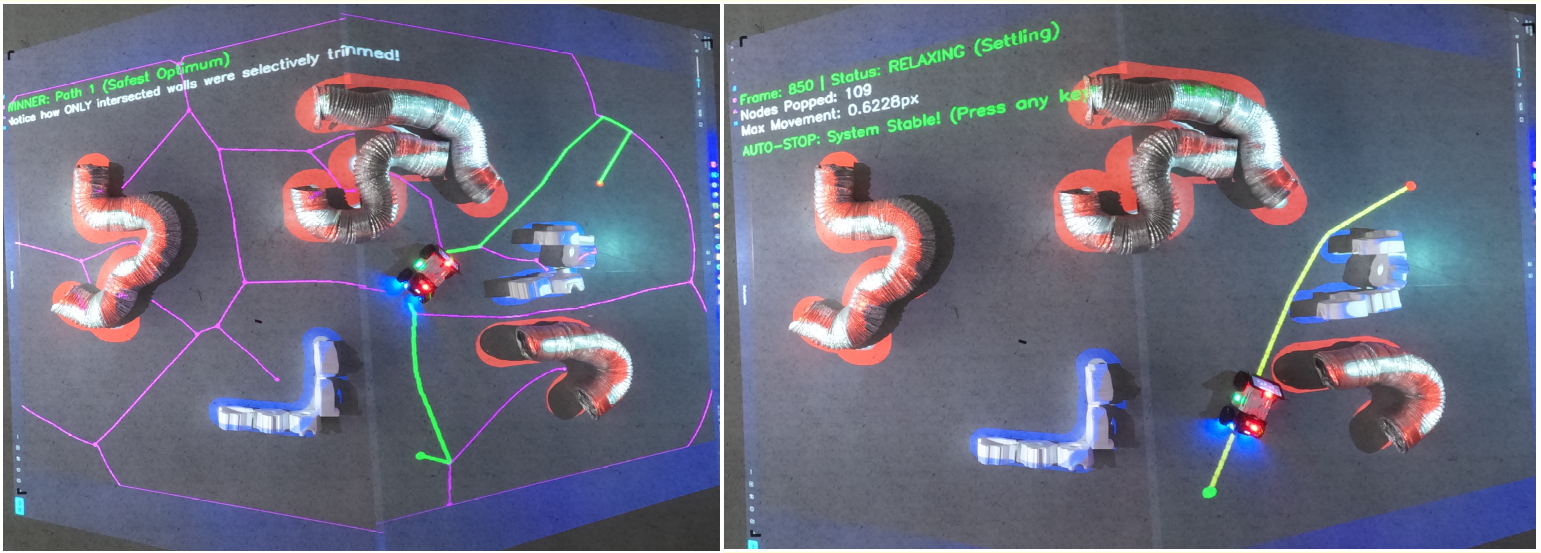
\includegraphics[width=\columnwidth]{hardware_omniwheel.png}}
\caption{Physical execution on an omnidirectional platform. The occupancy map, Topological Cage and planner state are projected onto the laboratory floor. \textbf{Left:} the cage (magenta) with the selected homotopy class shown as the raw skeletal route (green); clearance shells are thinned only on the obstacle components this route contacts, while others retain their nominal thresholds. \textbf{Right:} the same query after damped-band tensioning (yellow), settled by the kinetic auto-stop rule, with the robot tracking it through the relaxed bottleneck. \emph{The band rests against the selectively relaxed thresholds rather than being repelled out of them, and with a holonomic base the planned path is executed without a kinematic conversion stage.}}
\label{fig:hardware}
\end{figure}

% ==========================================
\section{Introduction}

Mobile robots in cluttered indoor environments repeatedly answer start-to-goal queries on a largely static map. Grid search (A$^\star$, Dijkstra) is resolution-complete but expands cells in proportion to free area, and because it minimizes length it hugs obstacle boundaries unless an inflation layer is hand-tuned. Sampling planners (PRM, RRT$^\star$) scale better in dimension, but narrow doorways and non-convex traps demand sampling densities that erode the advantage.

Distance-field skeletons invert this: precompute the locus of maximum clearance once, then route on it. This gives clearance by construction and a graph orders of magnitude smaller than the grid~\cite{lau2013,oleynikova2018,qi2022pruned}. Recent work makes the representation practical online, including incremental updates~\cite{lau2013} and, closest to our setting, the Enveloped Generalized Voronoi Graph (EGVG)~\cite{qi2025egvg}. Two problems remain.

\textbf{The injection problem.} A query point almost never lies on the skeleton. Nearest-pixel projection can cut through obstacles --- measured here at $2.1\%$ of terminals. Inserting the query as a temporary obstacle forces a local skeleton rebuild. Running A$^\star$ or BFS until a skeleton pixel is hit reintroduces grid expansion, at a cost that grows with distance to the skeleton, which is exactly the open-space case that dominates. Raycasting toward nearby vertices~\cite{qi2025egvg} is fast but its success depends on vertex placement.

\textbf{The Voronoi void.} In an expansive room, or around a free-standing island, the equidistance locus is sparse or forms a component disconnected from the rest. Over our four benchmarks the usable routing structure splits into $21$ components and the resulting planner declares only $24.0\%$ of queries feasible, though free space admits a solution for $93.0\%$.

Both defects share a root cause: the usable skeleton is an \emph{unbounded, possibly disconnected} set, while the query can be anywhere. Our response makes the routing structure \emph{bounded and connected by construction}. A tangent--gradient test identifies the structured interior and supplies the clearance scale $C_{\max}$; the ridge is truncated at $d_{\mathrm{cage}}=C_{\max}+\Delta$ and unioned with the level set $\{\Psi=d_{\mathrm{cage}}\}$. Truncation, not deletion, is what makes this work: the cut ends lie exactly on the level set and fasten its components into one structure. Gradient integration from any free point then meets the cage transversally, so injection succeeds without search. Map processing is paid once; each query costs a bounded number of gradient steps plus a search on a graph sized by topology, and the residual budget buys what per-query grid planners cannot afford --- enumerating $K$ topologically distinct routes and selecting by clearance rather than length. Fig.~\ref{fig:framework} summarizes the framework.

\textbf{Contributions.} (i) A bounded medial manifold from a tangent--gradient level-selection rule and a single super-critical level set, with a proof of connectedness, raising feasibility from $24.0\%$ to $99.6\%$ of attainable (Sec.~\ref{sec:offline}). (ii) A search-free bidirectional gradient injection whose termination follows from the eikonal property, attaching $100\%$ of terminals with zero connector collisions (Sec.~\ref{sec:online}). (iii) A lexicographic bottleneck criterion refining min-clearance selection, cutting ties by $56.7\%$ while raising mean clearance (Sec.~\ref{sec:opt}). (iv) A damped spring--mass band with per-obstacle relaxation, reducing integrated curvature by $85.2\%$ (Sec.~\ref{sec:opt}).

% ==========================================
\begin{figure}[!t]
\centerline{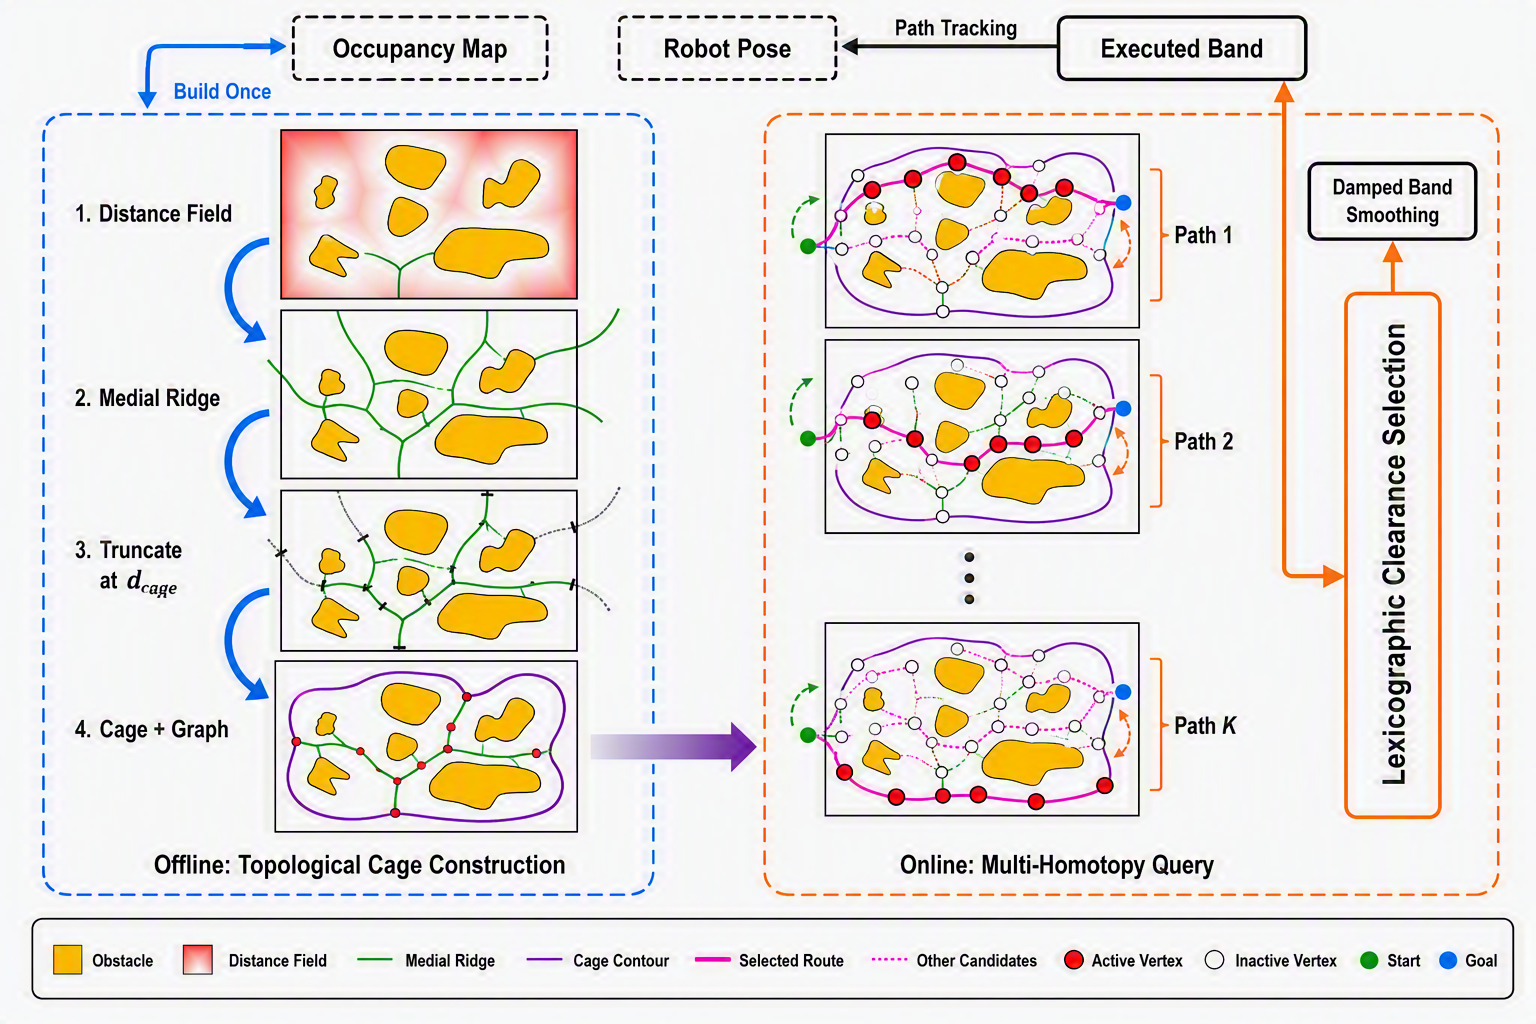
\includegraphics[width=\columnwidth]{Designer.png}}
\caption{Planning framework. \textbf{Left (offline, once per map):} the Euclidean distance field induces the medial ridge; the tangent--gradient test fixes the clearance scale $C_{\max}$, the ridge is truncated at $d_{\mathrm{cage}}=C_{\max}+\Delta$ --- the cut points, marked with ticks, lie exactly on the level set --- and the union with that level set yields the Topological Cage and its sparse graph. \textbf{Right (online, per query):} bidirectional gradient scouts attach start and goal without grid expansion, then $K$ candidates are enumerated on the graph. All candidates are superimposed in every panel; the route active in that panel is drawn bold with its committed vertices filled red, while inactive vertices remain hollow. Candidates differ in junction sequence, not local geometry, which is what makes them topologically distinct. The lexicographic clearance order then selects one route for damped-band smoothing. \emph{The entire left column is paid once; only the right column repeats per query.}}
\label{fig:framework}
\end{figure}

% ==========================================
\section{Related Work}

\textbf{Search, sampling and skeletons.} A$^\star$~\cite{hart1968} and replanning variants~\cite{koenig2005} are resolution-complete but expand cells proportional to explored area and are length- rather than clearance-optimal. PRM~\cite{kavraki1996} amortizes construction across queries --- the correct instinct --- but uniform sampling under-represents narrow passages, so the density needed for doorways inflates memory and construction cost. RRT$^\star$~\cite{karaman2011,lavalle1998} is asymptotically optimal but not naturally multi-query. Visibility graphs~\cite{yang2022far} and sparse roadmaps~\cite{dobson2014} shrink the graph but still grow with explored area. GVD/GVG methods instead extract the ridge set of the distance field~\cite{lau2013,hoff1999} and have served as RRT heuristics~\cite{chi2022}, AGV layers~\cite{zhang2024agv}, and aerial graphs~\cite{oleynikova2018}. Skeleton simplification by angle criteria is due to Foskey et al.~\cite{foskey2003}; our test is applied between skeleton tangent and distance gradient, and selects a clearance \emph{level} rather than discarding structure. EGVG~\cite{qi2025egvg} is closest, also adding distance-field contours, but differs in purpose and placement: it adds bands \emph{around obstacles} at a user-chosen $d_c$ for spatial expressiveness and connects terminals by raycasting to nearby vertices. We add \emph{one} contour at a level fixed by the map's own interior clearance scale, for topological closure, and use that closure to obtain a terminal connection needing no raycast, no obstacle insertion and no local search.

\textbf{Local optimization and homotopy selection.} DWA~\cite{fox1997} and TEB~\cite{rosmann2012} are the deployed standard; elastic bands~\cite{quinlan1993} balance contraction against repulsion. Two known failures motivate our variant: in tight corridors repulsion dominates contraction and the band freezes, and nodes without an enforced rest length slide and clump. Enumerating homotopy classes is established~\cite{bhattacharya2012,qi2025egvg}; EGVG enumerates by vertex suppression and selects by weighted length, heading deviation and path-change cost. We enumerate by $K$-shortest paths~\cite{yen1971} and select by a clearance-lexicographic order, optimizing safety first.

% ==========================================
\section{Problem Formulation}
\label{sec:problem}

Let $\mathcal{W}\subset\mathbb{R}^2$ be a bounded workspace on a grid of resolution $r$ (m/px), $\mathcal{O}$ the closed obstacle set, $\Omega=\mathcal{W}\setminus\mathcal{O}$ the open free set. The robot is a disc of radius $\rho$. Notation: $\Psi(p)$ is the Euclidean distance from $p$ to $\partial\mathcal{O}$ and $\hat{n}=\nabla\Psi/\|\nabla\Psi\|$; $\mathcal{M}$ is the medial ridge of $\Psi$ with unit tangent $\hat{t}_{\mathcal{M}}$; $\tau$ is the angular tolerance and $\mathcal{M}_{\mathrm{int}}$ the structured interior it selects; $C_{\max}=\sup_{\mathcal{M}_{\mathrm{int}}}\Psi$, $d_{\mathrm{cage}}=C_{\max}+\Delta$; $\mathcal{M}_{\mathrm{trunc}}=\{p\in\mathcal{M}:\Psi(p)\le d_{\mathrm{cage}}\}$, $\mathcal{B}=\{\Psi=d_{\mathrm{cage}}\}$, and the cage is $\mathcal{C}=\mathcal{M}_{\mathrm{trunc}}\cup\mathcal{B}$ with sparse graph $G=(V,E)$. Queries are $p_S,p_G$ with injection points $p_S',p_G'$; $\alpha$ is the integration step, $K$ the candidate count, $\sigma(P)$ the ascending-sorted clearance profile, $\tau_O$ the per-component repulsion threshold, and $\rho+\delta_{\mathrm{safe}}$ the hard safety floor.

\begin{assumption}
\label{asm:setting}
The map is static during a query batch, $\partial\mathcal{O}$ is known, and $\Omega$ is bounded and connected. $\Psi$ is computed by an exact Euclidean distance transform~\cite{felzenszwalb2012}, hence $1$-Lipschitz with $\|\nabla\Psi\|=1$ wherever differentiable. The offset is admissible: $C_{\max}<d_{\mathrm{cage}}<\sup_{\Omega}\Psi$.
\end{assumption}

Admissibility makes $\mathcal{B}$ non-empty and places it strictly above the interior structure; consequences are in Sec.~\ref{sec:limitations}.

Four problems follow. \textbf{(P1)} Attach $p_S,p_G\notin\mathcal{M}$ to the routing structure with cost independent of $|\Omega|$ and guaranteed rather than empirical success --- hard because $\mathcal{M}$ is measure-zero, so projection is unsafe and complete alternatives are searches. \textbf{(P2)} Build a connected superset of a possibly disjoint skeleton without heuristic bridging; failure means reporting infeasible for a feasible query, as EGVG does when terminals fall in different subgraphs~\cite{qi2025egvg}. \textbf{(P3)} Select the safest among $K$ routes under a deterministic total order, since minimum clearance alone ties frequently. \textbf{(P4)} Smooth the jagged skeletal route without triggering repulsion-dominance oscillation or node clumping. P1 and P2 are primary; P3 and P4 are enabled by the budget they release.

% ==========================================
\section{Offline Construction}
\label{sec:offline}

\subsection{Distance Field and Medial Ridge}

We compute the exact EDT of $\Omega$~\cite{felzenszwalb2012},
\begin{equation}
\Psi(p)=\min_{q\in\partial\mathcal{O}}\|p-q\|_2 ,
\end{equation}
with gradient by central differences. $\Psi$ solves the eikonal equation $\|\nabla\Psi\|=1$ on $\Omega\setminus\mathcal{M}$ and is non-differentiable precisely on $\mathcal{M}$, where the nearest-boundary point is non-unique and the gradient \emph{direction} jumps. The magnitude does not decay near $\mathcal{M}$ --- the property Sec.~\ref{sec:online} relies on. The medial set is the ridge,
\begin{equation}
\mathcal{M}=\{p\in\Omega \mid \exists\, p_i,p_j\in N(p):\ \nabla\Psi(p_i)\cdot\nabla\Psi(p_j)<0\},
\label{eq:ridge}
\end{equation}
with $N(p)$ the $8$-neighborhood, thinned to one pixel.

Two properties matter. $\mathcal{M}$ is a deformation retract of $\Omega$, hence \emph{connected} whenever $\Omega$ is. But it is \emph{unbounded in clearance}: it follows local clearance maxima into every open region, out to the widest parts of the map (Fig.~\ref{fig:raw_medial_axis}). The portion planners retain --- the structured corridors --- is what fragments into disconnected components.

\begin{figure}[htbp]
\centerline{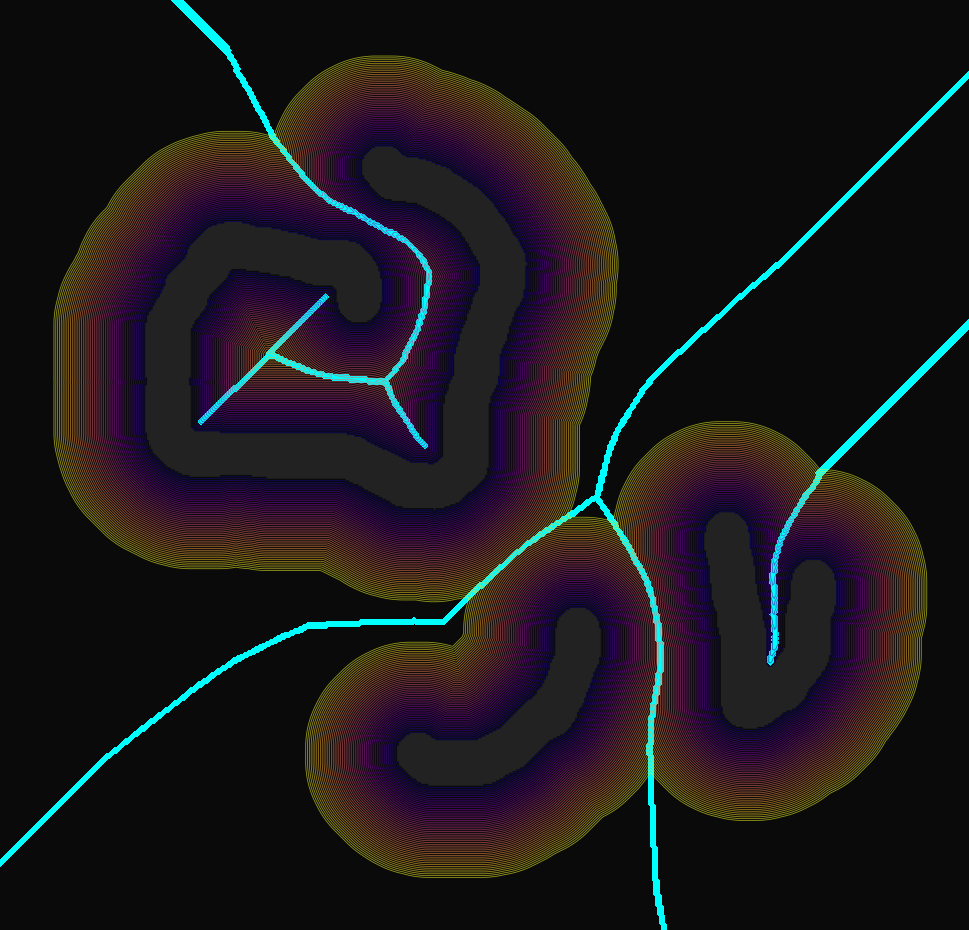
\includegraphics[width=0.85\columnwidth]{infinitemedial.png}}
\caption{Medial ridge (cyan). Interior corridors are captured correctly, but branches extend into open space toward the global clearance maxima, and structure around isolated obstacles forms loops with no corridor-level connection. \emph{The skeleton is connected but unbounded in clearance; retaining only its structured part is what fragments it.}}
\label{fig:raw_medial_axis}
\end{figure}

\subsection{Tangent--Gradient Test and Level Selection}

Inside a corridor the medial curve runs parallel to the flanking walls, so the gradient is near-orthogonal to the skeleton tangent; on a branch radiating into open space this breaks down. With $\theta(p)=|90^\circ-\arccos|\hat{t}_{\mathcal{M}}(p)\cdot\hat{n}(p)||$, the structured interior is
\begin{equation}
\mathcal{M}_{\mathrm{int}}=\big\{p\in\mathcal{M}\ \big|\ |\hat{t}_{\mathcal{M}}(p)\cdot\hat{n}(p)|\le \cos(90^\circ-\tau)\big\}.
\label{eq:prune}
\end{equation}
The projection is evaluated as the directional derivative of $\Psi$ along $\hat{t}_{\mathcal{M}}$, which is well defined on the ridge where $\nabla\Psi$ is not.

\textbf{This test selects a level, not a membership.} $\mathcal{M}_{\mathrm{int}}$ serves only to compute $C_{\max}$. Eq.~\eqref{eq:trunc} retains \emph{all} ridge points below the cage level, and exterior branches are truncated there rather than removed --- that distinction is what makes the construction connected. The test is local, costing $O(|\mathcal{M}|)$, and because the medial curve between two islands is locally still a corridor, the same threshold registers inter-island corridors as interior structure, so one scalar $\tau$ handles both wall and island topologies (Fig.~\ref{fig:angle_cutoff}). We use $\tau=17^\circ$; Sec.~\ref{sec:results} shows invariance over $[8^\circ,45^\circ]$.

\begin{figure}[htbp]
\centerline{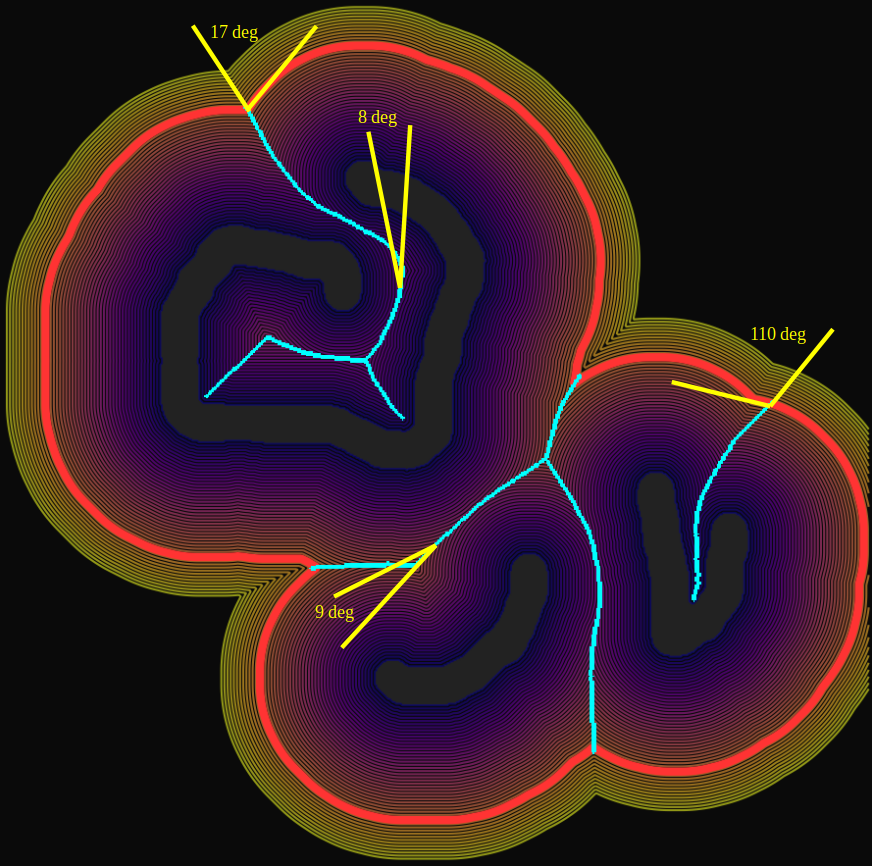
\includegraphics[width=0.85\columnwidth]{angleprunning.png}}
\caption{Tangent--gradient test. Interior corridors show near-orthogonal tangent/gradient pairs ($\theta\!\approx\!8^\circ$); branches into open space diverge ($\theta\!\approx\!110^\circ$) and fall outside $\mathcal{M}_{\mathrm{int}}$; the corridor between two free-standing islands stays parallel ($\theta\!\approx\!9^\circ$) and is registered by the same threshold.}
\label{fig:angle_cutoff}
\end{figure}

\subsection{Closure and Graph Abstraction}
\label{sec:closure}

With $C_{\max}=\sup_{p\in\mathcal{M}_{\mathrm{int}}}\Psi(p)$ and $d_{\mathrm{cage}}=C_{\max}+\Delta$ subject to Assumption~\ref{asm:setting},
\begin{align}
\mathcal{M}_{\mathrm{trunc}} &= \{p\in\mathcal{M}: \Psi(p)\le d_{\mathrm{cage}}\}, \label{eq:trunc}\\
\mathcal{B} &= \{p\in\Omega: |\Psi(p)-d_{\mathrm{cage}}|\le\varepsilon\},
\end{align}
with $\varepsilon$ half the grid diagonal, and
\begin{equation}
\boxed{\ \mathcal{C}=\mathcal{M}_{\mathrm{trunc}}\ \cup\ \mathcal{B}\ }
\label{eq:cage}
\end{equation}
$\mathcal{M}_{\mathrm{trunc}}$ is the \emph{full} ridge below the cage level, not $\mathcal{M}_{\mathrm{int}}$. Branches heading outward are cut where they cross $\Psi=d_{\mathrm{cage}}$ and kept up to that point; those cut ends lie on $\mathcal{B}$ and, by Theorem~\ref{thm:connected}, bind it into one structure. $\mathcal{M}_{\mathrm{trunc}}$ supplies clearance-maximal corridors where corridors exist; $\mathcal{B}$ supplies routing structure across open regions where the corridor notion degenerates. Unlike EGVG's user-chosen $d_c$ near obstacles, our single band sits at a level fixed by the map itself, because only a super-critical level yields the truncation geometry the proof needs.

\begin{figure}[htbp]
\centerline{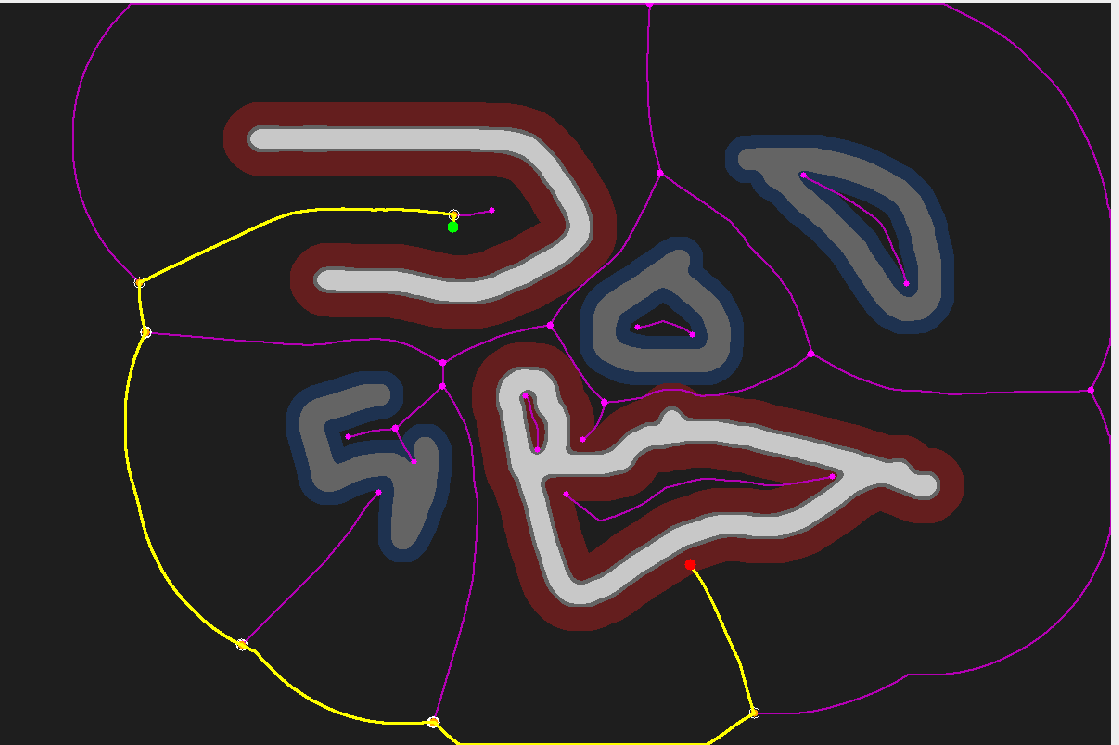
\includegraphics[width=0.95\columnwidth]{medialplusband.png}}
\caption{Assembled cage (purple) on a semantically annotated map; rigid (red) and deformable (blue) classes carry different clearance thresholds. The super-critical level set spans open regions and joins the truncated corridor systems into one connected manifold; a route is shown in yellow.}
\label{fig:semantic_cage}
\end{figure}

$\mathcal{C}$ compresses to $G=(V,E)$ by pixel-degree classification~\cite{qi2025egvg,lau2013}: degree $\ge 3$ are junctions, degree $1$ endpoints, degree $2$ edge interior; flood-fill along degree-$2$ chains yields edges, and nearby junctions are clustered. Pixels with $\Psi<\rho+\delta_{\mathrm{safe}}$ are discarded first, so every chain respects the safety floor and no edge-wise collision checking is needed at query time. Edge cost is accumulated axis displacement, $g(e)=\sqrt{a_x^2+a_y^2}$ with $a_d=\sum_k|d_{k+1}-d_k|$, and each edge stores its clearance profile. Graphs contain $44$--$116$ vertices on $375{,}000$-pixel maps --- roughly three orders of magnitude of compression, sized by topology rather than pixel count.

% ==========================================
\section{Online Query: Search-Free Injection}
\label{sec:online}

\subsection{Bidirectional Gradient Scouts}

From $p_S$ (identically $p_G$) we integrate
\begin{equation}
p_{k+1}=p_k \pm \alpha\,\hat{n}(p_k),
\label{eq:scout}
\end{equation}
terminating on contact with $\mathcal{C}$. The $+$ branch (``climber'') ascends toward higher clearance; the $-$ branch (``diver'') descends toward the nearest boundary.

Both are required for a structural reason. A terminal with $\Psi(p_S)<d_{\mathrm{cage}}$ lies below the envelope and ascending reaches either a corridor ridge or $\mathcal{B}$. A terminal with $\Psi(p_S)>d_{\mathrm{cage}}$ lies \emph{inside} an open region the envelope encircles; ascending climbs away from $\mathcal{B}$ toward a peak above the cage level, which is not in $\mathcal{C}$. Only descent recovers the envelope. Sec.~\ref{sec:results} measures this split directly. Both contacts are inserted into $G$ as temporary vertices and the search runs over the union, which additionally seeds distinct homotopy classes.

\begin{figure}[htbp]
\centerline{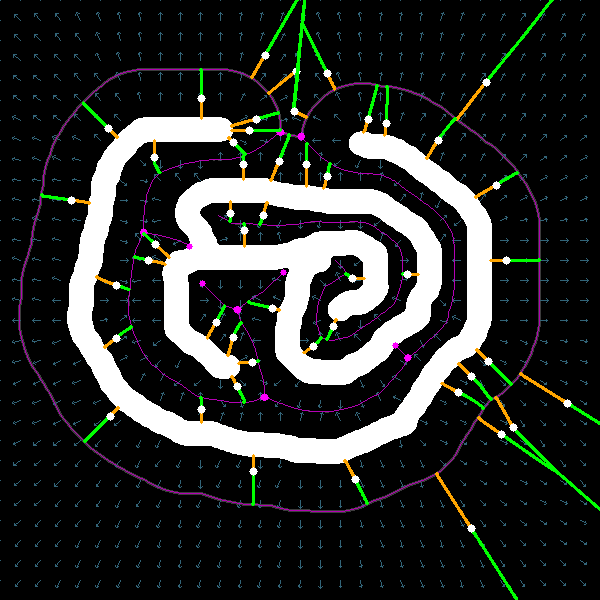
\includegraphics[width=0.85\columnwidth]{scout_navigation_map.png}}
\caption{Search-free injection. The climber (green) integrates $+\hat{n}$, the diver (orange) $-\hat{n}$, until contact with the cage (purple). Which branch succeeds is set by whether the terminal lies below or above the cage level.}
\label{fig:scouts}
\end{figure}

\subsection{Guarantees}

\begin{theorem}[Connectedness]
\label{thm:connected}
Under Assumption~\ref{asm:setting}, $\mathcal{C}=\mathcal{M}_{\mathrm{trunc}}\cup\mathcal{B}$ is connected.
\end{theorem}
\begin{proof}
$\mathcal{M}$ is a deformation retract of $\Omega$, hence connected. Let $\mathcal{B}_j$ be a component of $\{\Psi=d_{\mathrm{cage}}\}$ bounding a region $R_j$ on which $\Psi>d_{\mathrm{cage}}$; $R_j$ is non-empty by admissibility and bounded, and $\Psi$ is continuous on $\overline{R_j}$ with $\Psi=d_{\mathrm{cage}}$ on $\partial R_j$, so $\Psi$ attains an interior maximum in $R_j$. Every local maximum lies on $\mathcal{M}$, so $\mathcal{M}\cap R_j\neq\emptyset$; since $\mathcal{M}$ is connected and meets the sublevel region containing $\partial\mathcal{O}$, it crosses $\partial R_j=\mathcal{B}_j$, and at the crossing $\Psi=d_{\mathrm{cage}}$ exactly, so that point is in $\mathcal{M}_{\mathrm{trunc}}$ and on $\mathcal{B}_j$. Now take $p,q\in\mathcal{C}$ and $\gamma\subset\mathcal{M}$ joining them. Where $\Psi\circ\gamma\le d_{\mathrm{cage}}$, $\gamma$ lies in $\mathcal{M}_{\mathrm{trunc}}$. Each maximal excursion into $\{\Psi>d_{\mathrm{cage}}\}$ enters and leaves at level exactly $d_{\mathrm{cage}}$ on the same component $\mathcal{B}_j$, which is connected, so the two points are joined within $\mathcal{B}_j$. Replacing every excursion by the corresponding arc yields a path in $\mathcal{C}$.
\end{proof}

This is the formal content of P2: the cage unifies the interior structure rather than merely enclosing it.

\begin{theorem}[Finite-length injection]
\label{thm:injection}
For any $p_0\in\Omega$ with $\Psi(p_0)>\rho+\delta_{\mathrm{safe}}$, at least one of the two integral curves of $\pm\hat{n}$ from $p_0$ contacts $\mathcal{C}$ within arc length $|d_{\mathrm{cage}}-\Psi(p_0)|$.
\end{theorem}
\begin{proof}
Since $\Psi$ is eikonal, along $\dot{p}=\pm\hat{n}$ we have $\tfrac{d}{ds}\Psi=\pm 1$. The gradient magnitude does not decay toward $\mathcal{M}$; non-differentiability there is a jump in \emph{direction}. The curve therefore crosses $\mathcal{M}$ transversally at unit speed, and termination is by intersection rather than convergence. Monotonicity precludes cycles. If $\Psi(p_0)<d_{\mathrm{cage}}$ the climber either meets a ridge point at level $\le d_{\mathrm{cage}}$, which is in $\mathcal{M}_{\mathrm{trunc}}$ by Eq.~\eqref{eq:trunc}, or attains $d_{\mathrm{cage}}$ and meets $\mathcal{B}$. If $\Psi(p_0)>d_{\mathrm{cage}}$ the diver cannot reach $\partial\mathcal{O}$ without first attaining $d_{\mathrm{cage}}$, so it meets $\mathcal{B}$. The level changes at unit rate, giving the bound.
\end{proof}

No case needs a fallback traversal: because Eq.~\eqref{eq:trunc} retains every ridge point below the cage level, a scout terminating on a ridge terminates on the cage.

\begin{proposition}[Query cost]
Injection takes at most $\lceil |d_{\mathrm{cage}}-\Psi(p_0)|/\alpha \rceil$ constant-cost steps, independent of $|\Omega|$. Total query cost is $O(\Psi_{\text{span}}/\alpha) + O(K(|E|+|V|\log|V|))$~\cite{yen1971}, with $|V|,|E|$ set by topology rather than map area.
\end{proposition}

Because $\mathcal{C}$ and $G$ depend only on the map, they are shared across all queries and agents: a batch of $Q$ queries costs $T_{\mathrm{offline}}+Q\,T_{\mathrm{query}}$ rather than $Q\,T_{\mathrm{search}}$.

% ==========================================
\section{Selection and Smoothing}
\label{sec:opt}

\subsection{Enumeration and Lexicographic Selection}

With terminals inserted, we enumerate $K$ loopless shortest paths by Yen's algorithm~\cite{yen1971}, discarding candidates sharing more than a fixed fraction of edge weight with an accepted one, so the retained set spans distinct classes. $K$ bounds time, not structure: the procedure is monotone in $K$.

For $P$ with pixel sequence $\{p_1,\dots,p_M\}$, let $\sigma(P)=(\Psi_{(1)},\dots,\Psi_{(M)})$ sorted ascending. Define $P\succ P'$ iff $\sigma(P)$ is lexicographically greater, and select
\begin{equation}
P^\star=\arg\max\nolimits_{\succ}\ \{P_1,\dots,P_K\} .
\label{eq:lex}
\end{equation}
The first component is the minimum clearance, so \eqref{eq:lex} first maximizes the tightest passage --- the standard bottleneck objective, on which the two criteria agree exactly. The refinement acts on ties: when candidates share a tightest passage the order proceeds to the second-tightest. Comparison is $O(M)$ with early exit.

\begin{figure}[htbp]
\centerline{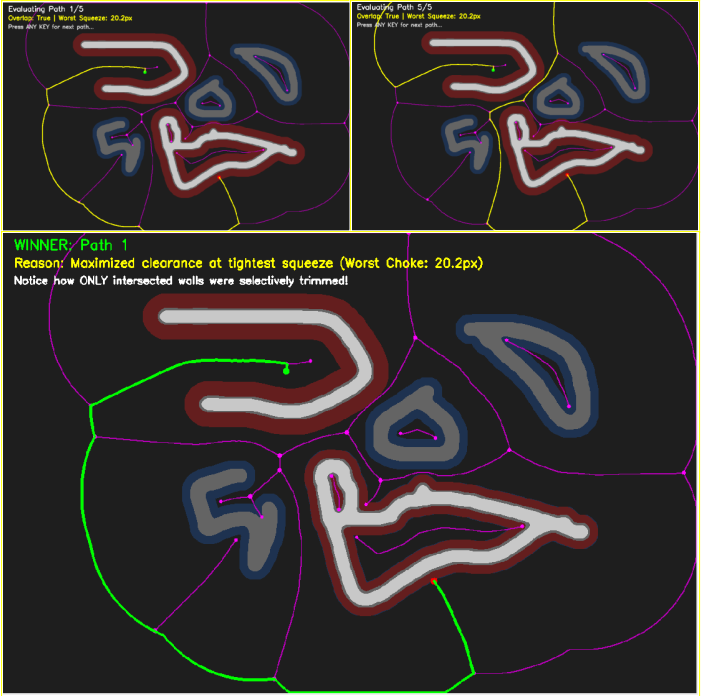
\includegraphics[width=\columnwidth]{pathcomp.png}}
\caption{Homotopy enumeration and lexicographic selection. Panels show $K$ topologically distinct candidates from both injection branches; annotations give the sorted clearance profile head. The selected route (bottom right) maximizes the tightest passage first and the second-tightest next, which is why it beats the geometrically shorter alternatives. \emph{Selection is by safety profile, not length, and the ordering is deterministic.}}
\label{fig:lexicographical}
\end{figure}

\subsection{Selective Relaxation and Damped Band}

A uniform repulsion threshold makes the band unable to enter any passage narrower than that threshold. Rather than lowering it globally, we lower it only where the route requires. Labelling obstacle components $\{O_1,\dots,O_m\}$ each with field $\Psi_O$, and recording $s_O=\min_{p\in P^\star}\Psi_O(p)$ for components the route intersects,
\begin{equation}
\tau_O=\min\big(\tau_O^{\mathrm{nom}},\ \max(s_O-\eta,\ \rho+\delta_{\mathrm{safe}})\big).
\label{eq:relax}
\end{equation}
Components off the route keep $\tau_O^{\mathrm{nom}}$. The clamp preserves safety: relaxation never falls below the robot radius plus margin, and a passage needing more is declined rather than executed (Sec.~\ref{sec:setup}).

Discretizing $P^\star$ into nodes $\{P_i\}$ with fixed endpoints,
\begin{equation}
\ddot{P}_i = W_s \vec{F}^{\,s}_i + W_r \vec{F}^{\,r}_i - D\,\dot{P}_i ,
\label{eq:dyn}
\end{equation}
\begin{equation}
\vec{F}^{\,s}_i=\!\!\sum_{j\in\{i\pm1\}}\!\!\frac{P_j-P_i}{\|P_j-P_i\|}\big(\|P_j-P_i\|-d_{\mathrm{rest}}\big),
\end{equation}
\begin{equation}
\vec{F}^{\,r}_i=\sum_{O} \frac{\nabla\Psi_O(P_i)}{\|\nabla\Psi_O(P_i)\|}\big[\tau_O-\Psi_O(P_i)\big]_+ ,
\end{equation}
so a node outside a threshold feels no force from that component. The rest length $d_{\mathrm{rest}}$ targets clumping: without it any node distribution is an equilibrium, so nodes drift and bunch. Damping removes the energy driving sustained oscillation between opposing walls; without it \eqref{eq:dyn} is conservative and the band does not settle. Integration is semi-implicit Euler with step $h$, and nodes are clamped to $\Psi(P_i)\ge\rho+\delta_{\mathrm{safe}}$ after each update.

\textbf{Distributed decimation.} Every $T_{\mathrm{pop}}$ iterations we delete every $N_{\mathrm{pop}}$-th node \emph{uniformly along the whole band}. Deleting from the ends instead tightens only terminal segments and leaves mid-path loops intact. \textbf{Stopping.} We track $v_{\max}=\max_i\|\dot{P}_i\|$ and stop when $v_{\max}<\epsilon_{\mathrm{stab}}$ for $n_{\mathrm{hold}}$ consecutive iterations, or at an iteration cap. Per-iteration cost is $O(N\cdot m_{\mathrm{active}})$ with $m_{\mathrm{active}}\le 3$ typically.

\begin{algorithm}[htbp]
\caption{Topological Cage query}
\label{alg:query}
\begin{algorithmic}[1]
\STATE \textbf{Offline:} $\Psi\!\leftarrow\!\mathrm{EDT}(\Omega)$; $\mathcal{M}\!\leftarrow\!\mathrm{ridge}(\Psi)$
\STATE $\mathcal{M}_{\mathrm{int}}\!\leftarrow\!$ Eq.~\eqref{eq:prune}; $C_{\max}\!\leftarrow\!\sup\Psi|_{\mathcal{M}_{\mathrm{int}}}$; $d_{\mathrm{cage}}\!\leftarrow\!C_{\max}\!+\!\Delta$
\STATE $\mathcal{C}\!\leftarrow\!\mathcal{M}_{\mathrm{trunc}}\cup\{\Psi\!=\!d_{\mathrm{cage}}\}$; $G\!\leftarrow\!\mathrm{abstract}(\mathcal{C})$
\STATE \textbf{Online:} integrate Eq.~\eqref{eq:scout} in $\pm$ from $p_S,p_G$; insert contacts
\STATE $\{P_1..P_K\}\leftarrow\mathrm{Yen}(G,p_S',p_G',K)$; $P^\star\leftarrow$ lex-max $\sigma(P_k)$
\STATE $\{\tau_O\}\leftarrow$ Eq.~\eqref{eq:relax} on $P^\star$
\STATE \textbf{if} all candidates need $\tau_O$ at floor \textbf{then return} unresolved
\STATE iterate Eq.~\eqref{eq:dyn} with decimation until $v_{\max}<\epsilon_{\mathrm{stab}}$
\end{algorithmic}
\end{algorithm}

% ==========================================
\section{Experimental Setup}
\label{sec:setup}

\textbf{Implementation.} Python (NumPy, OpenCV, NetworkX) on a single-threaded AMD Ryzen 5 5500U CPU (8GB RAM), using exact EDT~\cite{felzenszwalb2012} and Yen's algorithm~\cite{yen1971}. Fixed parameters for all runs: $\tau=17^\circ$, $\Delta=20$~px, $\alpha=0.5$~px, $K=5$, max overlap $0.85$, $r=0.02$~m/px, $\rho+\delta_{\mathrm{safe}}=6$~px ($0.12$~m), $\tau^{\mathrm{nom}}_{\mathrm{rigid}}=30$~px, $\tau^{\mathrm{nom}}_{\mathrm{soft}}=15$~px, $\eta=2$~px, $d_{\mathrm{rest}}=5$~px, initial spacing $8$~px, $W_s=0.55$, $W_r=2.5$, $D=0.4$, $h=1.0$, $\epsilon_{\mathrm{stab}}=0.7$~px/iter, $n_{\mathrm{hold}}=30$, $(N_{\mathrm{pop}},T_{\mathrm{pop}})=(10,20)$, $1500$ iteration cap.

\textbf{Environments.} Four $500\times750$~px benchmarks at $0.02$~m/px ($150$~m$^2$): \textbf{E1} (structured indoor, mixed obstacles), \textbf{E2} (semi-sparse, Voronoi-void stress case), \textbf{E3} (free-standing islands), and \textbf{E4} (U-shaped trap). Obstacles carry rigid/deformable labels with distinct thresholds. Three complex operator-drawn maps (spirals, concave islands, dense maze) serve as case studies.

\textbf{Resolution criterion.} A query is \emph{resolved} if $\ge 1$ candidate band solution maintains relaxed thresholds strictly above $\rho+\delta_{\mathrm{safe}}$. If all candidates require relaxation below this safety floor, the planner deliberately reports \emph{unresolved} to avoid unsafe narrow gaps. All baselines are scored against this same floor.

\textbf{Baselines.} Grid A$^\star$~\cite{hart1968} (also used as an oracle to normalize feasibility of reachable pairs); PRM~\cite{kavraki1996} ($2500$ samples, $k=12$, doorway-tuned); RRT$^\star$~\cite{karaman2011} ($0.05$ goal bias); GVD routing with A$^\star$ terminal connection; and a DWA-style planner~\cite{fox1997} for trap studies. EGVG's raycast connection mechanism is evaluated as ablation A2c.

\textbf{Protocol.} Evaluated on $Q=100$ randomized start--goal pairs per environment ($400$ total), sampled uniformly in free space ($\Psi>\rho+\delta_{\mathrm{safe}}$, distance $\ge 120$~px). We use $200$ additional terminals per environment for injection stats, $320$ for branch attachment, $40$ queries for band ablations, and $375$ multi-candidate queries for selection stats.

\textbf{Hardware.} An omnidirectional platform tracked by overhead motion capture (Fig.~\ref{fig:hardware}). The map, cage, scouts, and elastic band are projected onto the laboratory floor. Planar paths are published as \texttt{nav\_msgs/Path} and directly executed via a holonomic velocity controller without kinematic conversion.

% ==========================================
\section{Results}
\label{sec:results}

\subsection{Overall Comparison}

Table~\ref{tab:master} evaluates cost and feasibility across $400$ randomized queries (E1--E4) and an independent maze benchmark.

Feasibility distinguishes the methods sharply: GVD with A$^\star$ connection resolves only $33.5\%$ due to skeleton disconnections, while our caged routing hits $92.8\%$. Our routing stage takes $24.7$~ms against A$^\star$'s $250.2$~ms ($10.1\times$ faster). Over $100$ queries, our total time (including offline cost) is $2.81$~s vs.\ A$^\star$'s $25.02$~s (break-even at $2$ queries). PRM is faster ($8.2$~ms) but requires $945.5$~ms offline, resolves only $84.3\%$, and ignores corridor clearance. In the maze benchmark, our planner visits just $98$ nodes compared to $244{,}021$ for A$^\star$ and $360{,}000$ for FMM, while uniquely maintaining $14$~px clearance from boundaries.

\begin{table*}[htbp]
\caption{Consolidated comparison. Left: E1--E4 ($Q=400$). Right: maze case study. Best per column in bold.}
\label{tab:master}
\begin{center}
\begin{tabular}{@{}l cccc c cccc@{}}
\toprule
& \multicolumn{4}{c}{\textbf{Benchmark suite E1--E4 ($Q=400$)}} & & \multicolumn{4}{c}{\textbf{Maze case study (single query)}} \\
\cmidrule(lr){2-5} \cmidrule(lr){7-10}
\textbf{Method} & \textbf{Offline} & \textbf{Query} & \textbf{Total 100q} & \textbf{Resolved} & & \textbf{Nodes/cells} & \textbf{Clearance} & \textbf{Time} & \textbf{Success} \\
 & (ms) & (ms) & (s) & (\%) & & \textbf{visited} & (px) & (ms) & \\ \midrule
A$^\star$~\cite{hart1968}              & $\mathbf{0.0}$ & $250.2$ & $25.02$ & $\mathbf{93.0}$ & & $244{,}021$ & $1.0$ & $3695.99$ & yes \\
RRT$^\star$~\cite{karaman2011}         & $\mathbf{0.0}$ & $117.6$ & $11.76$ & $92.5$ & & $1{,}191$ & $0.0$ & $473.77$ & no \\
PRM (dense)~\cite{kavraki1996}         & $945.5$ & $\mathbf{8.2}$ & $1.77$ & $84.3$ & & $1{,}002$ & $3.0$ & $430.76$ & yes \\
FMM                                    & --- & --- & --- & --- & & $360{,}000$ & $0.0$ & $176.22$ & no \\
GVD + A$^\star$ inject                 & $114.7$ & $17.4$ & $1.85$ & $33.5$ & & --- & --- & --- & --- \\ \midrule
\textbf{Ours} (global routing)         & $343.9$ & $24.7$ & $\mathbf{2.81}$ & $92.8$ & & $\mathbf{98}$ & $\mathbf{14.0}$ & $\mathbf{28.38}$ & \textbf{yes} \\
\textbf{Ours} (routing $+$ band)       & $343.9$ & $84.7$ & $8.81$ & $92.8$ & & --- & --- & --- & --- \\ \bottomrule
\end{tabular}
\end{center}
\footnotesize Band stage outputs an executable smoothed trajectory. Routing row is the like-for-like global-planning comparison. Normalized against A$^\star$ attainability, our feasibility is $99.6\%$ (Table~\ref{tab:perenv}).
\end{table*}

\subsection{Per-Environment Evidence}

Table~\ref{tab:perenv} details environmental performance. Caging reduces the raw $21$ disconnected components down to $5$ (E2--E4 condense to a single component each, fulfilling Theorem~\ref{thm:connected}). Consequently, raw feasibility leaps from $24.0\%$ to $92.8\%$.

The most dramatic improvements align with theoretical expectations: in open (E2) and free-standing (E3) maps, uncaged feasibility is $7\%$ and $13\%$, while the cage hits $100\%$. In E1, sealed walls cap theoretical attainability at $72\%$; our planner resolves $71\%$. Across all $400$ queries, our method missed only one attainable path. Query times show enumeration dominates ($22.13$~ms) compared to injection ($2.16$~ms). Graph sizes ($44$--$116$ vertices) scale with topology, not map area.

\begin{table}[htbp]
\caption{Per-environment closure, feasibility, graph size, and query cost}
\label{tab:perenv}
\begin{center}
\setlength{\tabcolsep}{3.5pt}
\begin{tabular}{@{}lcccccccc@{}}
\toprule
& \multicolumn{2}{c}{\textbf{Components}} & \multicolumn{3}{c}{\textbf{Feasibility (\%)}} & \multicolumn{3}{c}{\textbf{Query cost (ms)}} \\
\cmidrule(lr){2-3} \cmidrule(lr){4-6} \cmidrule(lr){7-9}
\textbf{Env} & raw & caged & attain. & raw & caged & inject & enum & tension \\ \midrule
E1 & $8$ & $2$ & $72$ & $25.0$ & $71.0$ & $1.49$ & $30.83$ & $63.78$ \\
E2 & $4$ & $\mathbf{1}$ & $100$ & $7.0$ & $\mathbf{100.0}$ & $4.43$ & $15.97$ & $45.86$ \\
E3 & $6$ & $\mathbf{1}$ & $100$ & $13.0$ & $\mathbf{100.0}$ & $1.60$ & $28.01$ & $42.71$ \\
E4 & $3$ & $\mathbf{1}$ & $100$ & $51.0$ & $\mathbf{100.0}$ & $1.12$ & $13.71$ & $61.93$ \\ \midrule
Mean & $21$ & $\mathbf{5}$ & $93$ & $24.0$ & $\mathbf{92.8}$ & $2.16$ & $22.13$ & $53.57$ \\ \bottomrule
\end{tabular}
\end{center}
\footnotesize Graph sizes $|V|/|E|$: E1 $116/163$, E2 $52/75$, E3 $75/114$, E4 $44/61$. Normalized feasibility (caged $\div$ attainable) averages $99.6\%$. Costs exclude overheads from Table~\ref{tab:sweep}.
\end{table}

\subsection{Component Contributions}

Table~\ref{tab:ablation} isolates each claim.

\textbf{Closure and injection.} Skeleton closure is critical; routing on the truncated skeleton alone drops feasibility to $26.3\%$. For injection, our gradient method uniquely achieves $100\%$ attachment with zero collisions. Nearest-pixel matches attachment but routes $2.1\%$ of connectors through obstacles. A$^\star$ is safe but scales poorly with distance to the skeleton ($2{,}443$ cell expansions vs.\ our $60.7$ integration steps). EGVG's raycast is fastest ($0.079$~ms) but its attachment drops to $93.5\%$ in E4 due to line-of-sight failures.

\textbf{Bidirectional scouts.} Results validate the partition in Theorem~\ref{thm:injection}. In structured maps (E1, E3, E4), the climber attaches $100\%$ of terminals. In open space (E2), the climber attaches $73.8\%$ and the diver $27.5\%$ (averaging $74.6$ descent steps). The branches overlap on only $1.3\%$ of terminals, confirming that bidirectionality effectively partitions the space and resolves the open-space Voronoi void problem.

\textbf{Selection and band.} Lexicographic and max-min-clearance criteria yield identical minimum clearance ($1.001$~m), outperforming shortest-length selection by $3.0\%$. Lexicographic refinement further reduces ties ($247\rightarrow107$) and improves mean clearance ($1.557\rightarrow1.588$~m). The full elastic band cuts integrated curvature by $85.2\%$, angular jerk by $74.8\%$, and spacing dispersion by $97.4\%$, while shortening path length by $20.3\%$. Damping is critical: omitting it spikes curvature $39\times$ and leaves only $2.5\%$ of runs settled. Selective relaxation cuts curvature by $37.6\%$ and improves settling ($67.5\rightarrow83.8\%$). 

In the E4 trap ($33$ trials), a myopic planner failed $33/33$ times, while both RRT$^\star$ and our pipeline succeeded $33/33$. However, unlike RRT$^\star$, which returns any valid homotopy class (often grazing boundaries), our method strictly guarantees route selection via clearance profiles.

\begin{table}[htbp]
\caption{Component contributions (mean over E1--E4)}
\label{tab:ablation}
\begin{center}
\setlength{\tabcolsep}{4pt}
\begin{tabular}{@{}llccc@{}}
\toprule
\textbf{ID} & \textbf{Variant} & \textbf{Feas.\ \%} & \textbf{Min clr (m)} & \textbf{Cost} \\ \midrule
A1 & no closure & $26.3$ & $0.910$ & $45.4$~ms \\ \midrule
\multicolumn{5}{@{}l}{\textit{A2 --- injection mechanism (attachment \%, collisions)}} \\
A2a & nearest-pixel & $100.0$ & \multicolumn{2}{c}{$2.1\%$ collide, $0.879$~ms} \\
A2b & A$^\star$ to skeleton & $100.0$ & \multicolumn{2}{c}{$2443$ cells, $3.182$~ms} \\
A2c & raycast~\cite{qi2025egvg} & $98.4$ & \multicolumn{2}{c}{$0\%$ collide, $\mathbf{0.079}$~ms} \\
-- & \textbf{gradient (ours)} & $\mathbf{100.0}$ & \multicolumn{2}{c}{$\mathbf{0\%}$ collide, $60.7$ steps} \\ \midrule
\multicolumn{5}{@{}l}{\textit{A3 --- scout branches (attachment over 320 terminals)}} \\
A3 & climber only & $93.4$ & $0.870$ & $83.8$\% routed \\
A3 & diver only & $9.1$ & --- & $0.0$\% routed \\
-- & \textbf{both} & $\mathbf{100.0}$ & $0.854$ & $\mathbf{94.4}$\% routed \\ \midrule
\multicolumn{5}{@{}l}{\textit{A4 --- selection criterion (375 multi-candidate queries)}} \\
A4 & shortest length & $0.972$ & $1.530$ mean & $1$ tie \\
A4 & max min-clr & $\mathbf{1.001}$ & $1.557$ mean & $247$ ties \\
-- & \textbf{lexicographic} & $\mathbf{1.001}$ & $\mathbf{1.588}$ mean & $\mathbf{107}$ ties \\ \midrule
\multicolumn{5}{@{}l}{\textit{A5 --- band terms ($\int|\kappa|ds$, spacing CV, settled \%)}} \\
A5 & raw skeletal & $26.96$ & $3.810$ & --- \\
A5 & no damping & $155.11$ & $0.648$ & $2.5$ \\
A5 & no relaxation & $5.48$ & $0.185$ & $67.5$ \\
A5 & end decimation & $3.94$ & $0.174$ & $\mathbf{86.9}$ \\
A5 & no rest length & $\mathbf{2.77}$ & $0.153$ & $70.6$ \\
-- & \textbf{full} & $3.98$ & $\mathbf{0.101}$ & $83.8$ \\ \bottomrule
\end{tabular}
\end{center}
\footnotesize A3 per-environment attachment: climber $100/73.8/100/100$, diver $1.3/\mathbf{27.5}/3.8/3.8$, either $100$ throughout. Only E2 places terminals above $d_{\mathrm{cage}}$ in quantity.
\end{table}

\subsection{Parameter Sensitivity and Complex Environments}

Table~\ref{tab:sweep} sweeps the four free parameters. Feasibility remains invariant ($91.3\%$) across wide ranges of $\tau\in[8^\circ,45^\circ]$ and $\Delta\in[5,80]$~px, confirming the construction is robust to these constants within the admissible range of Assumption~\ref{asm:setting}. Clearance saturates at $K=3$, allowing a $40\%$ reduction in the enumeration budget without quality loss. Injection achieves $100\%$ attachment across $\alpha\in[0.25,4.0]$~px; running at $\alpha=4.0$ reduces integration cost $6.9\times$ with no measured penalty.

\begin{table}[htbp]
\caption{Parameter sensitivity, mean over E1--E4}
\label{tab:sweep}
\begin{center}
\setlength{\tabcolsep}{2pt}
\begin{tabular}{@{}lccccc@{}}
\toprule
\textbf{$\tau$ (deg)} & $8$ & $12$ & $17$ & $30$ & $45$ \\
Feas.\ \% / min clr & $91.3/.901$ & $91.3/.863$ & $91.3/.854$ & $91.3/.841$ & $91.3/.839$ \\ \midrule
\textbf{$\Delta$ (px)} & $5$ & $10$ & $20$ & $40$ & $80$ \\
Feas.\ \% / min clr & $91.3/.886$ & $91.3/.852$ & $91.3/.854$ & $91.3/.850$ & $91.3/.884$ \\ \midrule
\textbf{$K$} & $1$ & $3$ & $5$ & $8$ & $12$ \\
Query ms / min clr & $41.0/.839$ & $61.1/.854$ & $62.2/.854$ & $62.2/.854$ & $61.9/.854$ \\ \midrule
\textbf{$\alpha$ (px)} & $0.25$ & $0.5$ & $1.0$ & $2.0$ & $4.0$ \\
Attach \% / steps & $100/123.6$ & $100/62.5$ & $100/32.0$ & $100/16.7$ & $\mathbf{100/9.1}$ \\ \bottomrule
\end{tabular}
\end{center}
\footnotesize $|V|$ varies $68.0$--$73.0$ over the $\tau$ sweep and $69.5$--$72.3$ over $\Delta$. Query times here include graph-copy and attachment overhead excluded from Table~\ref{tab:perenv}.
\end{table}

Fig.~\ref{fig:casestudy} demonstrates the pipeline on three complex, operator-drawn maps with high branching and boundary curvature. In all cases, the cage unified the skeleton into a single routing manifold, terminals injected seamlessly, and the lexicographic criterion successfully selected a winner from $K=5$ candidates. Selective relaxation visually thins clearance shells exactly where the route contacts them. Fig.~\ref{fig:hardware} displays the corresponding physical execution: the omnidirectional platform tracking the tensioned, settled band.


\begin{figure*}[htbp]
\centerline{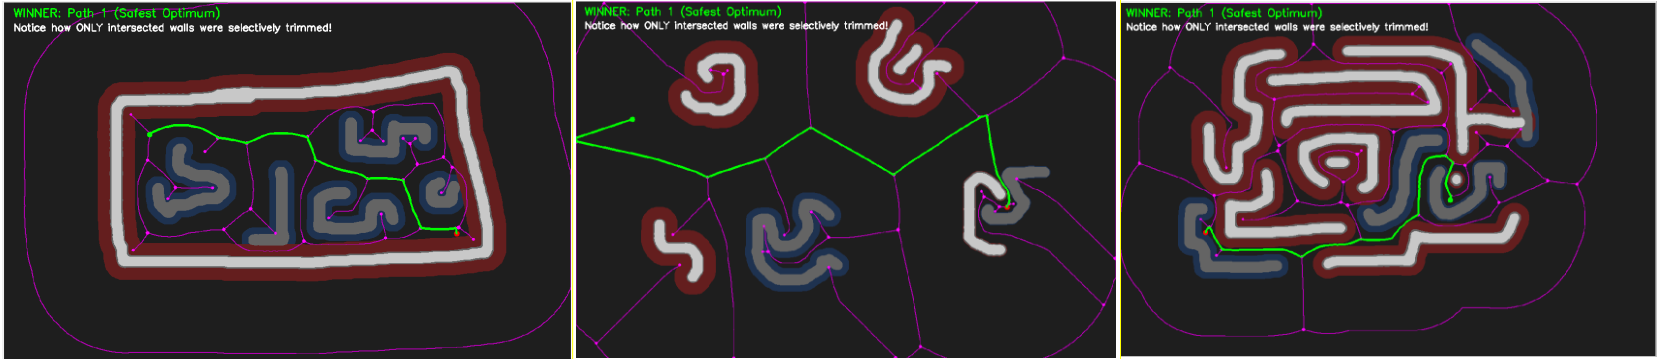
\includegraphics[width=0.96\textwidth]{E134.png}}
\caption{Pipeline on three operator-drawn environments of higher geometric complexity than the benchmark suite. Left: nested spiral corridors with mixed rigid (grey/red) and deformable (blue) semantic boundaries. Centre: five free-standing islands with concave cavities. Right: dense multi-branch maze. In all three the cage (magenta) unifies the skeleton into one routing manifold, both terminals inject without grid expansion, $K=5$ distinct homotopy classes are enumerated, and the lexicographic criterion selects the green route. Clearance shells are thinned only on components the route actually contacts. \emph{Enumeration, selection and per-component relaxation behave as specified well beyond the benchmark suite.}}
\label{fig:casestudy}
\end{figure*}

% ==========================================
\section{Limitations and Future Work}
\label{sec:limitations}

\textbf{Global scalar cage level.} $d_{\mathrm{cage}}$ relies on $C_{\max}$, a global supremum. A single wide hallway pushes the envelope outward workspace-wide. This restricts admissibility (Assumption~\ref{asm:setting}: if the tangent--gradient test admits too much open space, $C_{\max}$ peaks and $\mathcal{B}$ empties) and limits the cage to static maps, as local edits globally alter the envelope. Spatially varying cage levels indexed by local clearance statistics would address this.

\textbf{Discretization sensitivity.} Lexicographic comparison depends on the exact global minimum $\Psi_{(1)}$, making the bottleneck objective vulnerable to grid aliasing. Quantile-based comparisons or profile smoothing trade exact guarantees for robustness.

\textbf{Safety floor scope.} Clamping nodes to $\Psi\ge\rho+\delta_{\mathrm{safe}}$ ensures safety only discretely; interpolated trajectories require swept-segment tests. Additionally, $\Psi$ models circular footprints; non-convex bodies require C-space distance fields or inscribed-disc approximations. Kinodynamic limits are deferred downstream.

\textbf{Narrow-passage refusal.} The planner conservatively rejects paths requiring relaxation below the safety floor, bypassing narrow gaps an aggressive kinodynamic planner might otherwise navigate.

\textbf{Future work.} Enumeration via Yen's algorithm currently generates redundant paths that require post-filtering. Because the cage graph is small, topologically abstract, and carries precomputed edge profiles, future work should enumerate directly on the vertex sequence. Suppressing junction vertices instead of edges places each successor in a distinct homotopy class by construction. This yields a topologically complete, non-redundant candidate set while eliminating the primary computational bottleneck in query cost.
% ==========================================
\section{Conclusion}

We presented the Topological Cage, a bounded medial manifold built by truncating the medial axis at a clearance level fixed by a tangent--gradient test and unioning it with the distance level set at that value. The construction is connected by proof: the truncation points of the ridge lie on the level set and pin its components together, so the cage unifies the routing structure rather than merely enclosing it. Empirically this reduces components from $21$ to $5$ across four benchmarks and raises feasibility from $24.0\%$ to $99.6\%$ of attainable. Because the distance field is eikonal, injection is a transversal crossing rather than a convergence, attaching $100\%$ of terminals with zero connector collisions in $60.7$ steps against $2{,}443$ expansions for the search-based fallback. The resulting cost structure breaks even against A$^\star$ after two queries and funds homotopy enumeration with lexicographic clearance selection, plus a damped band that cuts curvature by $85.2\%$ while retaining a hard safety floor. Three complex operator-drawn environments and hardware trials on an omnidirectional platform confirm the behaviour, and parameter sweeps show feasibility invariant across wide ranges of $\tau$, $\Delta$, $K$ and $\alpha$. Generating successor routes by suppressing junction vertices of the cage graph, rather than edges of a pixel-level path, would make the candidate set topologically complete and, given how small the graph is, cheaper than the procedure used here.

% ==========================================
\appendices
\section{The Voronoi Void}
\label{appendix:voronoi_void}

In a large open region the structured-corridor interpretation of the medial axis degenerates: the nearest boundaries are far apart and the equidistance locus is sparse, offering no usable routing structure at the scale a robot needs (Fig.~\ref{fig:voronoi_problem}). Around a free-standing obstacle the failure differs in kind --- the skeleton forms a closed loop \emph{around} the obstacle, a legitimate structure with no corridor-level connection to the rest. Both are measurable: in E2 the uncaged structure splits into four components and resolves $7\%$ of queries; in E3, five islands, six components and $13\%$.

\begin{figure}[htbp]
\centerline{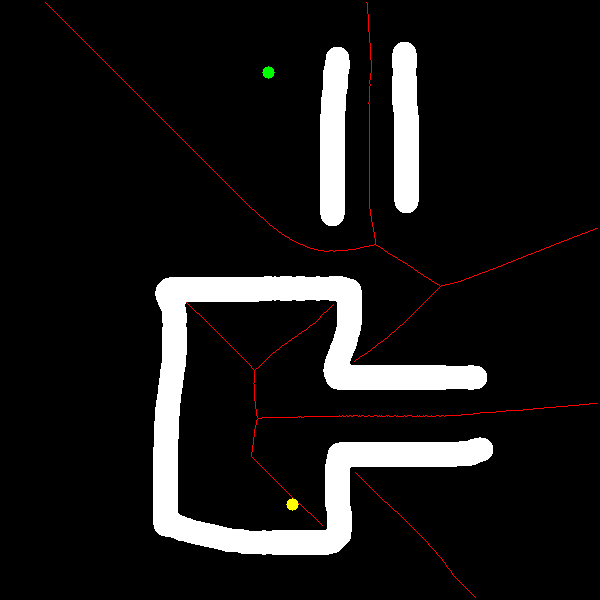
\includegraphics[width=0.8\columnwidth]{voronoi_shortcoming_raw.png}}
\caption{Voronoi void. The standard medial axis (red) provides no usable structure across the open region, leaving the query point (green) with nothing to connect to. \emph{The failure is in the representation, not the connection procedure.}}
\label{fig:voronoi_problem}
\end{figure}

The standard recourse is a grid search until a skeleton pixel is found, whose cost grows with the size of the void --- precisely the wrong scaling, confirmed by the $3{,}068$ versus $2{,}031$ expansion asymmetry between E2 and E1. The cage removes the need: $\mathcal{B}$ passes through the open region by construction because $\Psi$ attains $d_{\mathrm{cage}}$ there, and gradient integration reaches that level within arc length $|d_{\mathrm{cage}}-\Psi(p_0)|$ (Fig.~\ref{fig:voronoi_resolution}).

\begin{figure}[htbp]
\centerline{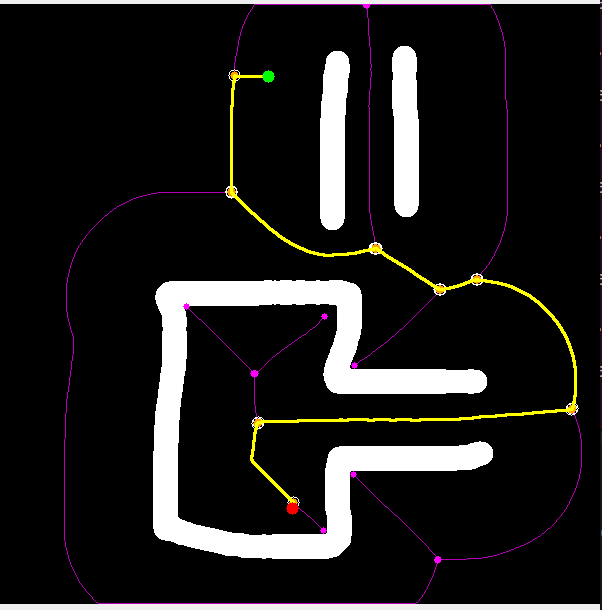
\includegraphics[width=0.8\columnwidth]{voronoi_our_path.png}}
\caption{Resolution by closure. The cage (purple) crosses the open region; the scout reaches it by monotone gradient integration and the query routes on the unified structure (yellow) with no grid expansion.}
\label{fig:voronoi_resolution}
\end{figure}

% ==========================================
\begin{thebibliography}{00}
\bibitem{qi2025egvg} H. Qi \emph{et al.}, ``Enveloped Generalized Voronoi Graph and multi-topology path planning for navigation in unknown environments,'' \textit{TechRxiv preprint}, Oct.\ 2025, doi:10.36227/techrxiv.176159300.02637396/v1.
\bibitem{hart1968} P. E. Hart, N. J. Nilsson, and B. Raphael, ``A formal basis for the heuristic determination of minimum cost paths,'' \textit{IEEE Trans. Syst. Sci. Cybern.}, vol. 4, no. 2, pp. 100--107, 1968.
\bibitem{koenig2005} S. Koenig and M. Likhachev, ``Fast replanning for navigation in unknown terrain,'' \textit{IEEE Trans. Robot.}, vol. 21, no. 3, pp. 354--363, 2005.
\bibitem{kavraki1996} L. E. Kavraki \emph{et al.}, ``Probabilistic roadmaps for path planning in high-dimensional configuration spaces,'' \textit{IEEE Trans. Robot. Autom.}, vol. 12, no. 4, pp. 566--580, 1996.
\bibitem{lavalle1998} S. M. LaValle, ``Rapidly-exploring random trees: A new tool for path planning,'' Tech. Rep. TR 98-11, Iowa State Univ., 1998.
\bibitem{karaman2011} S. Karaman and E. Frazzoli, ``Sampling-based algorithms for optimal motion planning,'' \textit{Int. J. Robot. Res.}, vol. 30, no. 7, pp. 846--894, 2011.
\bibitem{felzenszwalb2012} P. F. Felzenszwalb and D. P. Huttenlocher, ``Distance transforms of sampled functions,'' \textit{Theory of Computing}, vol. 8, no. 1, pp. 415--428, 2012.
\bibitem{lau2013} B. Lau, C. Sprunk, and W. Burgard, ``Efficient grid-based spatial representations for robot navigation in dynamic environments,'' \textit{Robot. Auton. Syst.}, vol. 61, no. 10, pp. 1116--1130, 2013.
\bibitem{hoff1999} K. E. Hoff III \emph{et al.}, ``Fast computation of generalized Voronoi diagrams using graphics hardware,'' in \textit{Proc. SIGGRAPH}, 1999, pp. 277--286.
\bibitem{oleynikova2018} H. Oleynikova \emph{et al.}, ``Sparse 3D topological graphs for micro-aerial vehicle planning,'' in \textit{IEEE/RSJ IROS}, 2018, pp. 1--9.
\bibitem{qi2022pruned} Y. Qi \emph{et al.}, ``Compact and efficient topological mapping for large-scale environment with pruned Voronoi diagram,'' \textit{Drones}, vol. 6, no. 7, p. 183, 2022.
\bibitem{foskey2003} M. Foskey, M. C. Lin, and D. Manocha, ``Efficient computation of a simplified medial axis,'' in \textit{Proc. ACM Symp. Solid Modeling}, 2003, pp. 96--107.
\bibitem{chi2022} W. Chi \emph{et al.}, ``A generalized Voronoi diagram-based efficient heuristic path planning method for RRTs in mobile robots,'' \textit{IEEE Trans. Ind. Electron.}, vol. 69, no. 5, pp. 4926--4937, 2022.
\bibitem{zhang2024agv} R. Zhang \emph{et al.}, ``Design and practical implementation of a high efficiency two-layer trajectory planning method for AGV,'' \textit{IEEE Trans. Ind. Electron.}, vol. 71, no. 2, pp. 1811--1822, 2024.
\bibitem{yang2022far} F. Yang \emph{et al.}, ``FAR planner: Fast, attemptable route planner using dynamic visibility update,'' in \textit{IEEE/RSJ IROS}, 2022, pp. 9--16.
\bibitem{dobson2014} A. Dobson and K. E. Bekris, ``Sparse roadmap spanners for asymptotically near-optimal motion planning,'' \textit{Int. J. Robot. Res.}, vol. 33, no. 1, pp. 18--47, 2014.
\bibitem{quinlan1993} S. Quinlan and O. Khatib, ``Elastic bands: Connecting path planning and control,'' in \textit{IEEE ICRA}, 1993, pp. 802--807.
\bibitem{rosmann2012} C. R\"osmann \emph{et al.}, ``Trajectory modification considering dynamic constraints of autonomous robots,'' in \textit{7th German Conf.\ Robotics}, 2012, pp. 1--6.
\bibitem{fox1997} D. Fox, W. Burgard, and S. Thrun, ``The dynamic window approach to collision avoidance,'' \textit{IEEE Robot. Autom. Mag.}, vol. 4, no. 1, pp. 23--33, 1997.
\bibitem{yen1971} J. Y. Yen, ``Finding the $k$ shortest loopless paths in a network,'' \textit{Management Science}, vol. 17, no. 11, pp. 712--716, 1971.
\bibitem{bhattacharya2012} S. Bhattacharya, M. Likhachev, and V. Kumar, ``Topological constraints in search-based robot path planning,'' \textit{Autonomous Robots}, vol. 33, no. 3, pp. 273--290, 2012.
\end{thebibliography}

\end{document}

